\section{Results and Discussion}

We measure the performance of proofreading quantitatively by comparing VI scores of segmentations against ground truth labelings. Lower VI scores indicate less distance to the ground truth and a better segmentation. For all experiments, we report the VI score of the initial segmentation followed by the VI score of the proofreading output.

\subsection{Selection Oracle}

\subsection{Automatic Method}

\subsection{Force Choice User Experiment}

The initial segmentation for AC4 had a VI of XXX. 

\textbf{Novice Performance.} 
\\~\\
\textbf{Expert Performance.}
\\~\\
\textbf{Subjective Responses.} All subjective responses were recorded using the NASA-TLX workload index. The workload index asks study participants to state their mental, physical, temporal demands, as well as rate their performance, effort, and frustration on a scale with 21 graduations. Mental, physical, and temporal demands were reported slightly higher for participants using focused proofreading. However, these differences were not statistically significant. This is not surprising since the user interface was the same for both control groups.

\begin{figure*}
    \centering
    \begin{subfigure}[b]{0.24\textwidth}
        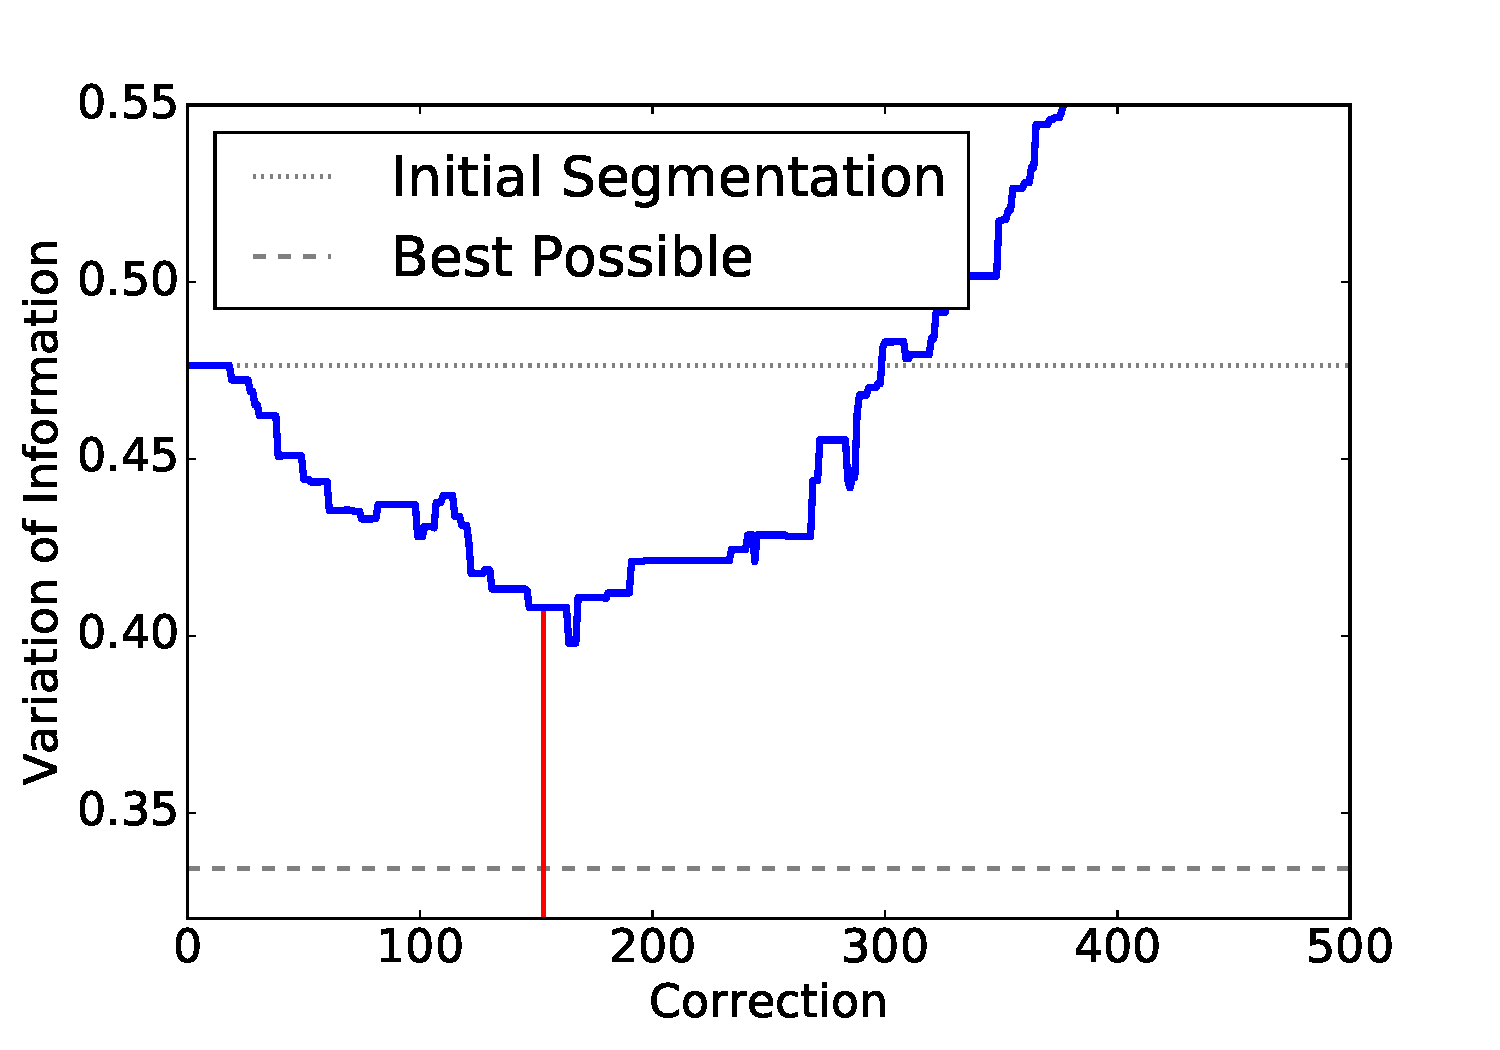
\includegraphics[width=\textwidth]{gfx/gpauto.pdf}
        \caption{A gull}
        \label{fig:gull}
    \end{subfigure}
    ~ %add desired spacing between images, e. g. ~, \quad, \qquad, \hfill etc. 
      %(or a blank line to force the subfigure onto a new line)
    \begin{subfigure}[b]{0.24\textwidth}
        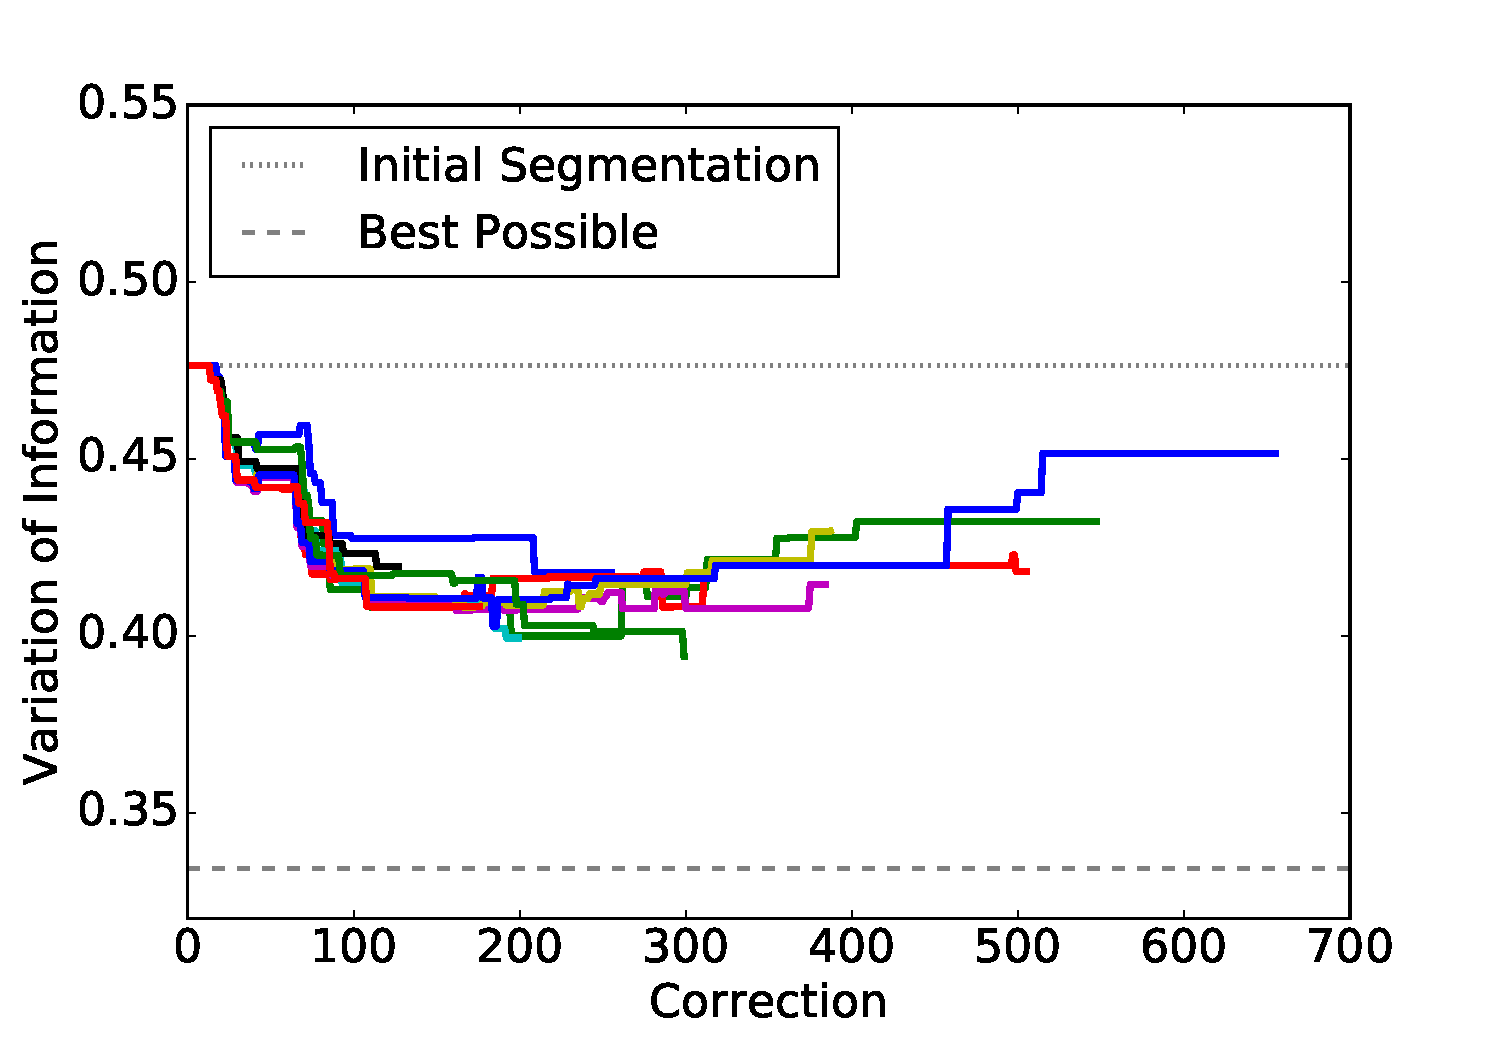
\includegraphics[width=\textwidth]{gfx/gpusers.pdf}
        \caption{A tiger}
        \label{fig:tiger}
    \end{subfigure}
    \begin{subfigure}[b]{0.24\textwidth}
        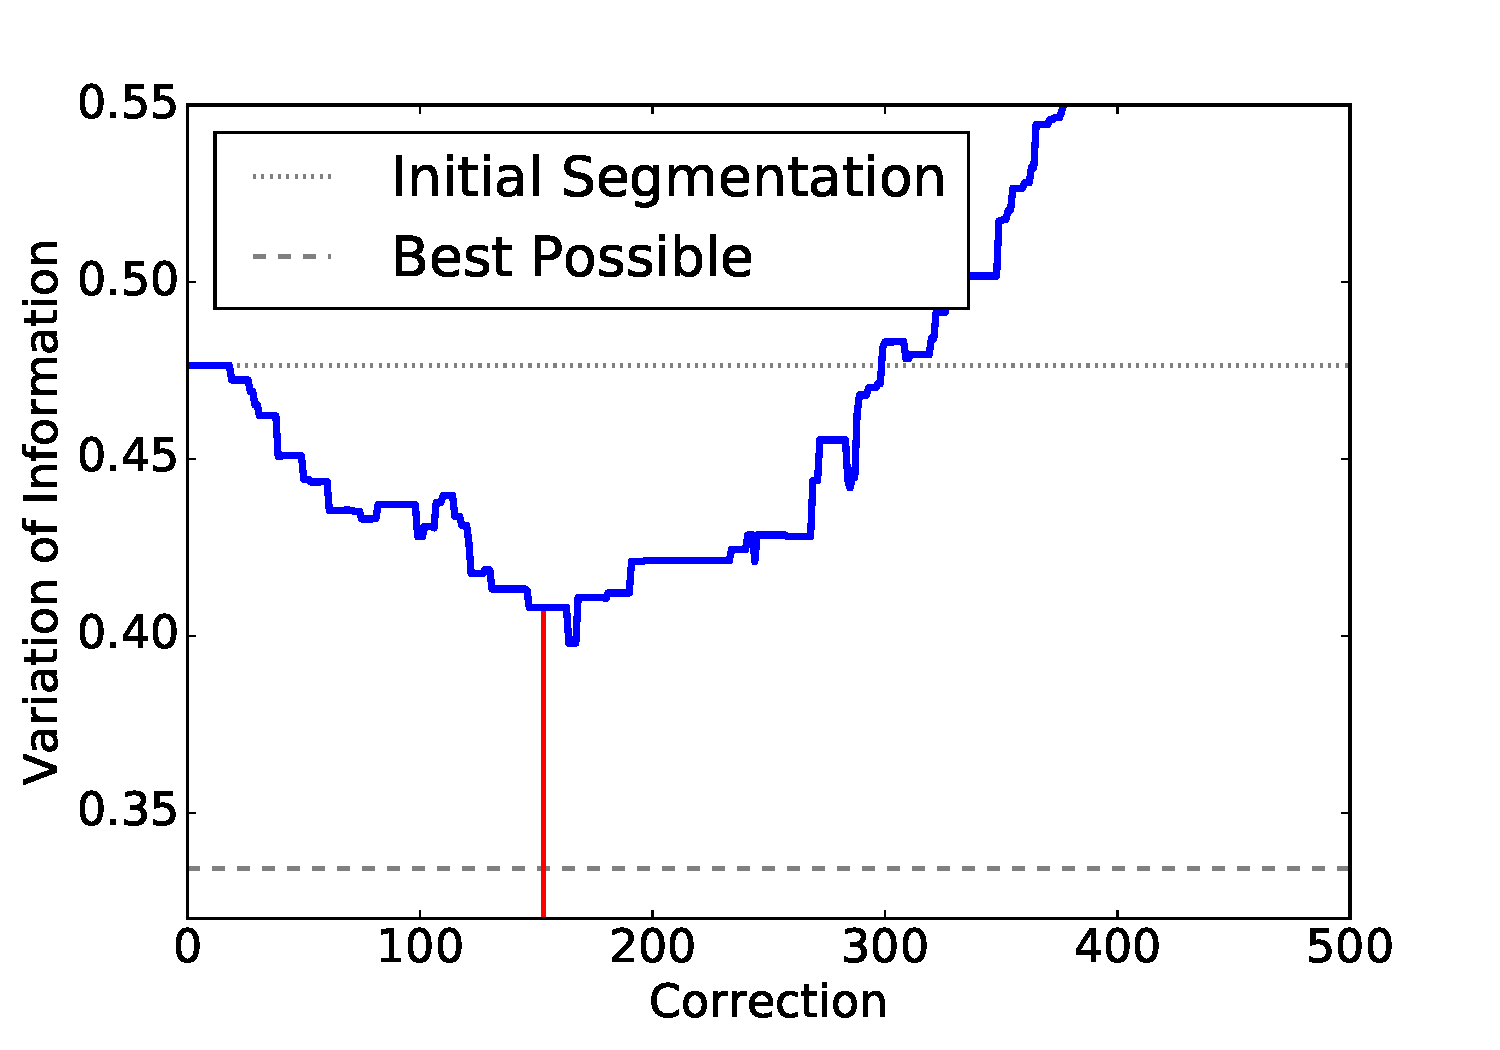
\includegraphics[width=\textwidth]{gfx/gpauto.pdf}
        \caption{A gull}
        \label{fig:gull}
    \end{subfigure}
    ~ %add desired spacing between images, e. g. ~, \quad, \qquad, \hfill etc. 
      %(or a blank line to force the subfigure onto a new line)
    \begin{subfigure}[b]{0.24\textwidth}
        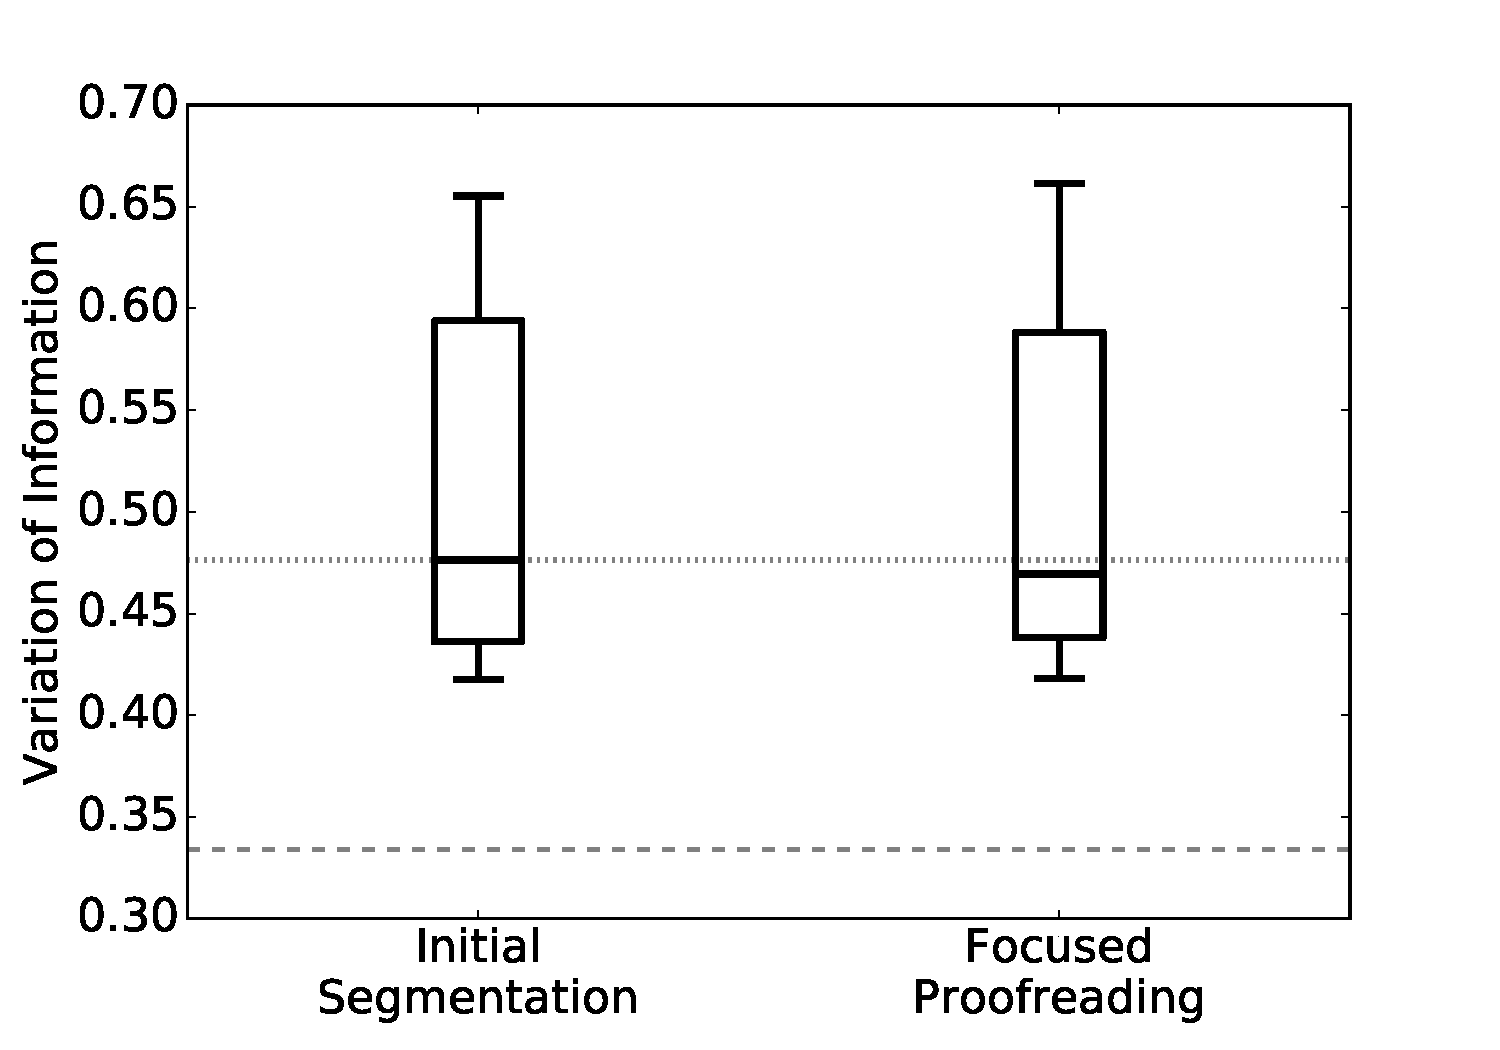
\includegraphics[width=\textwidth]{gfx/fc_fp_ac4.pdf}
        \caption{A tiger}
        \label{fig:tiger}
    \end{subfigure}
    ~ %add desired spacing between images, e. g. ~, \quad, \qquad, \hfill etc. 
    %(or a blank line to force the subfigure onto a new line)
%    \begin{subfigure}[b]{0.15\textwidth}
%        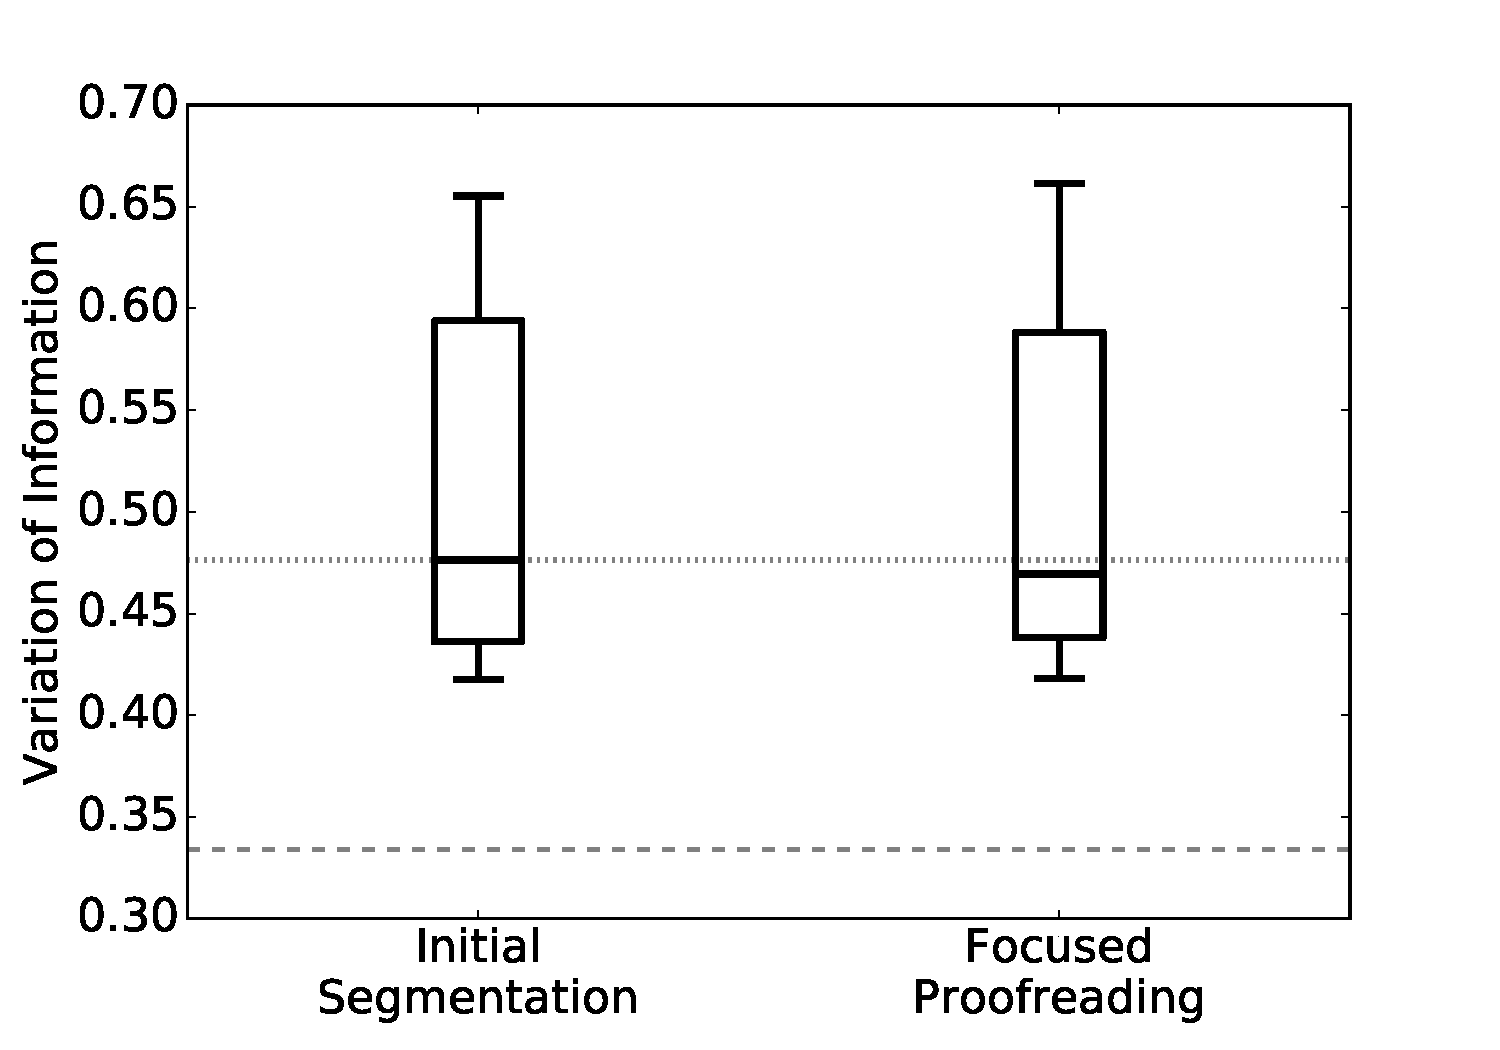
\includegraphics[width=\textwidth]{gfx/fc_fp_ac4.pdf}
%        \caption{A mouse}
%        \label{fig:mouse}
%    \end{subfigure}
    \caption{Pictures of animals}\label{fig:animals}
\end{figure*}
\begin{figure}
    \centering
    \begin{subfigure}[b]{0.48\linewidth}
        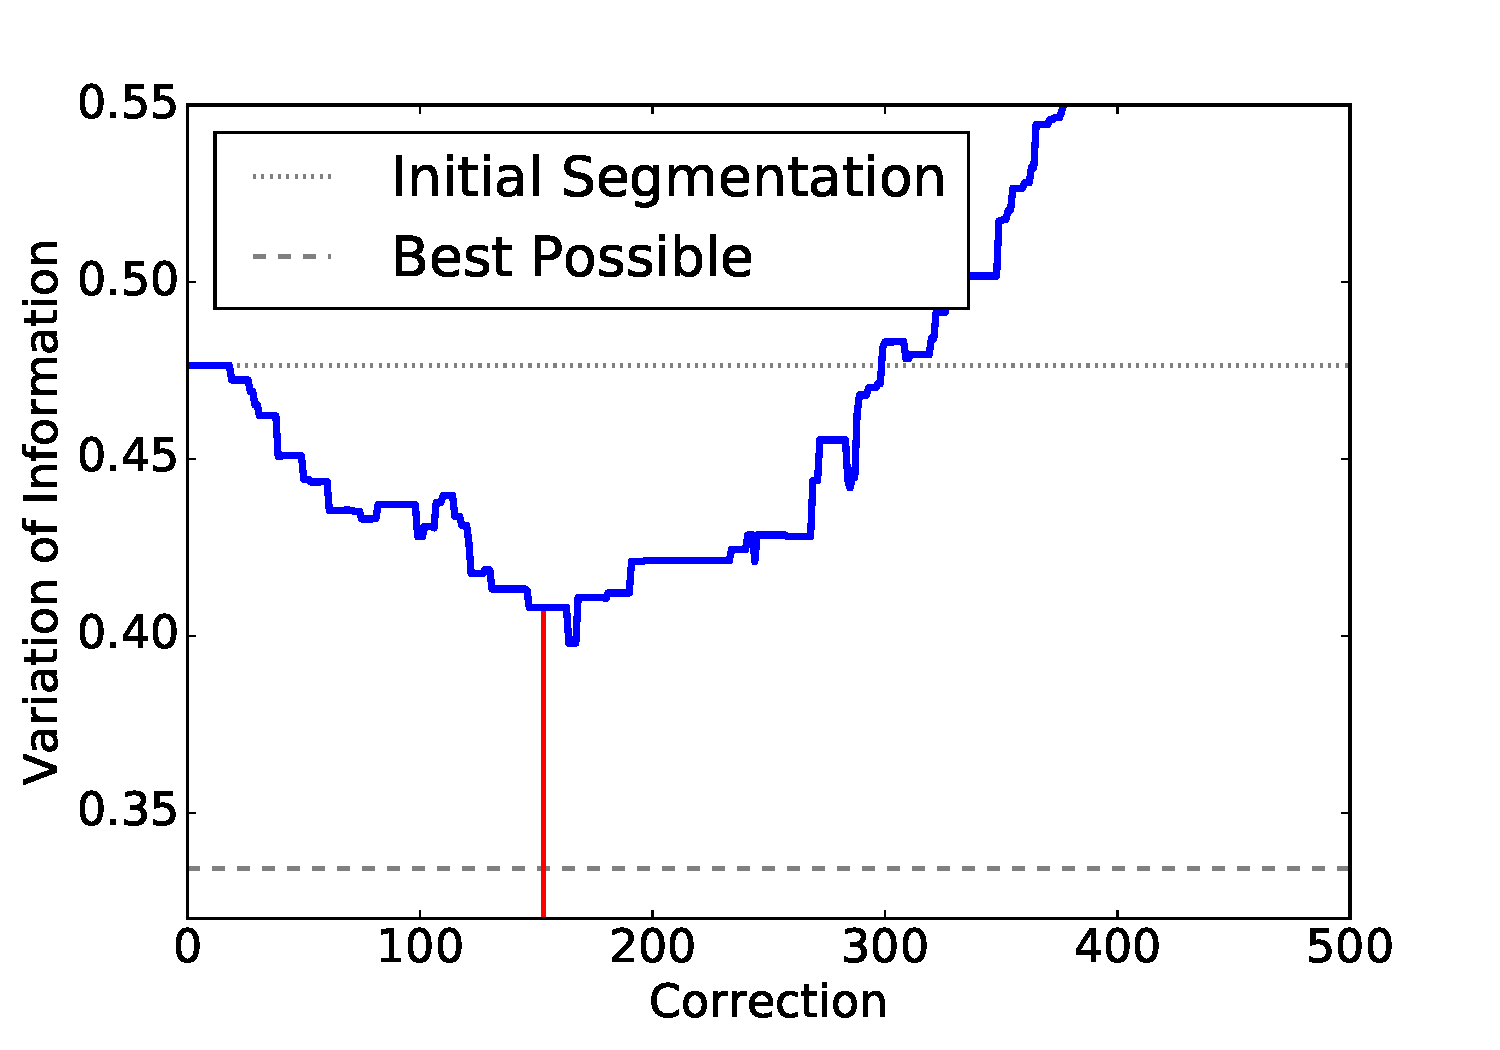
\includegraphics[width=\textwidth]{gfx/gpauto.pdf}
        \caption{A gull}
        \label{fig:gull}
    \end{subfigure}
    ~ %add desired spacing between images, e. g. ~, \quad, \qquad, \hfill etc. 
      %(or a blank line to force the subfigure onto a new line)
    \begin{subfigure}[b]{0.49\linewidth}
        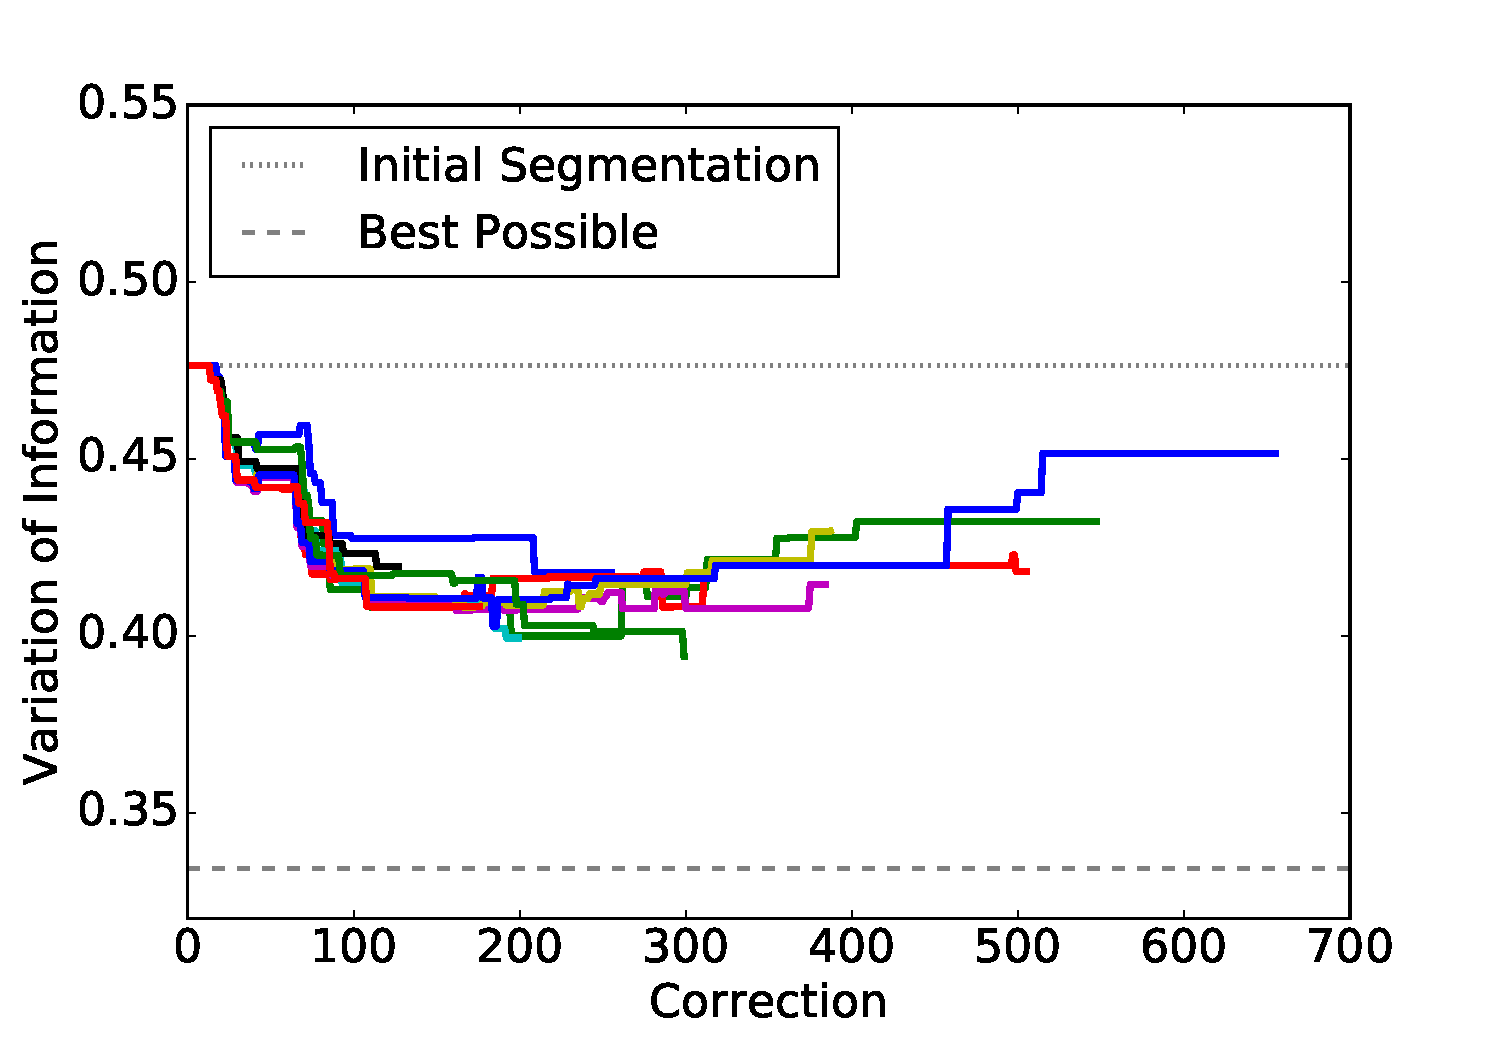
\includegraphics[width=\textwidth]{gfx/gpusers.pdf}
        \caption{A tiger}
        \label{fig:tiger}
    \end{subfigure}
    ~ %add desired spacing between images, e. g. ~, \quad, \qquad, \hfill etc. 
    %(or a blank line to force the subfigure onto a new line)
%    \begin{subfigure}[b]{0.15\textwidth}
%        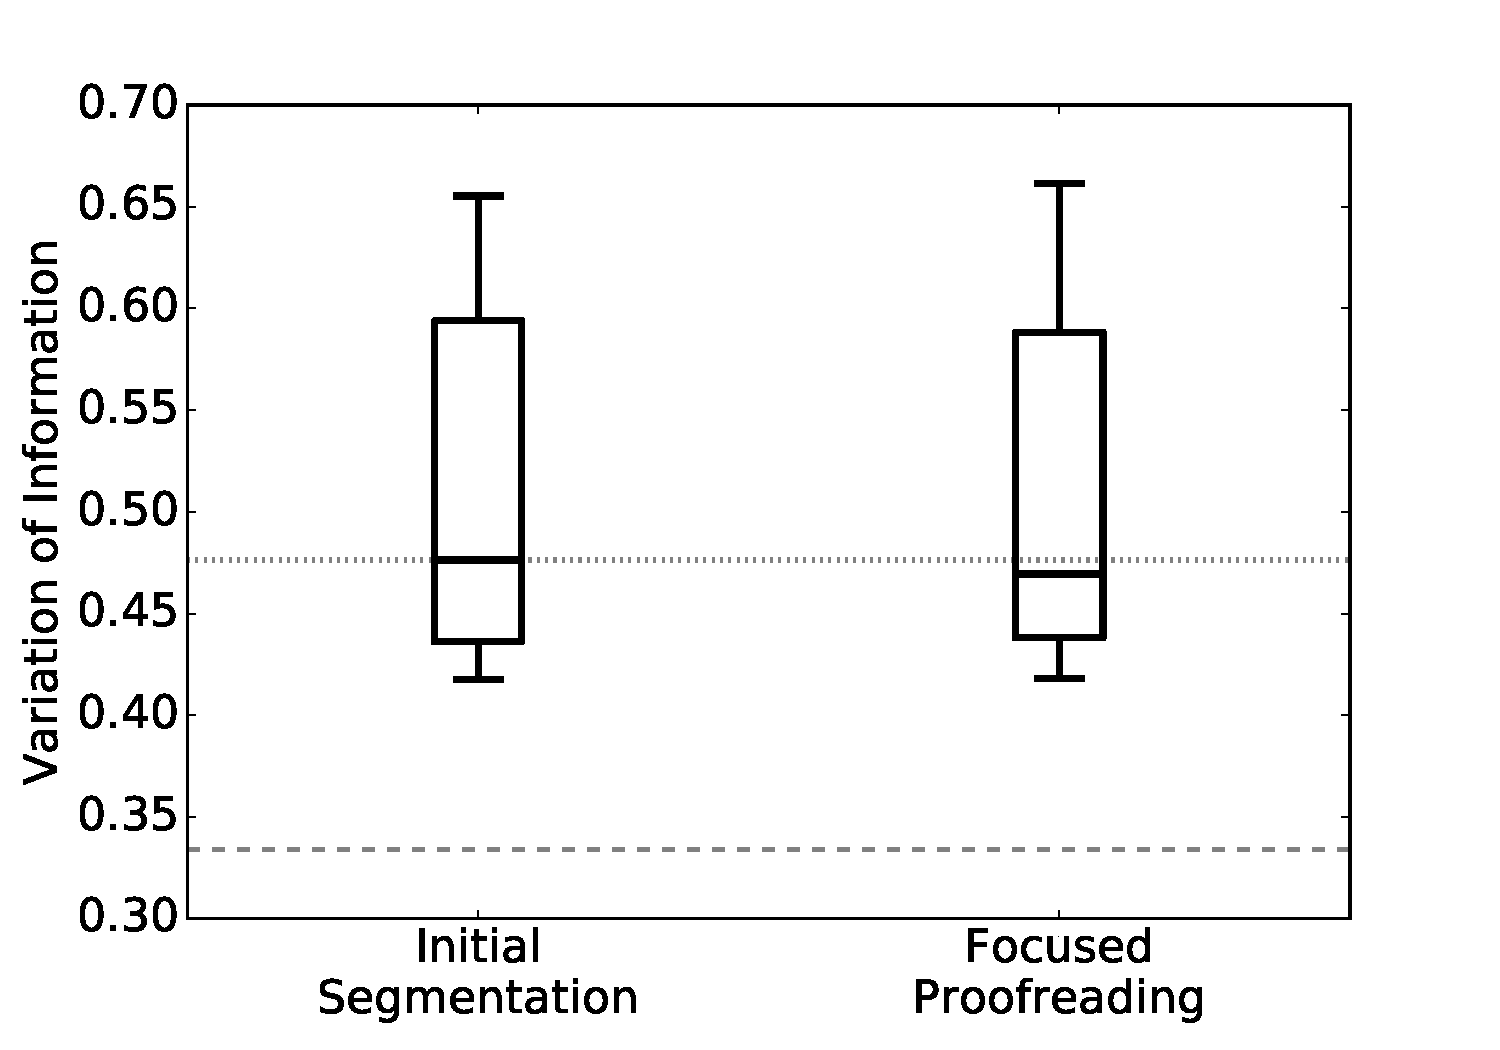
\includegraphics[width=\textwidth]{gfx/fc_fp_ac4.pdf}
%        \caption{A mouse}
%        \label{fig:mouse}
%    \end{subfigure}
    \caption{Pictures of animals}\label{fig:animals}
\end{figure}

\begin{figure}
    \centering
    \begin{subfigure}[b]{0.49\linewidth}
        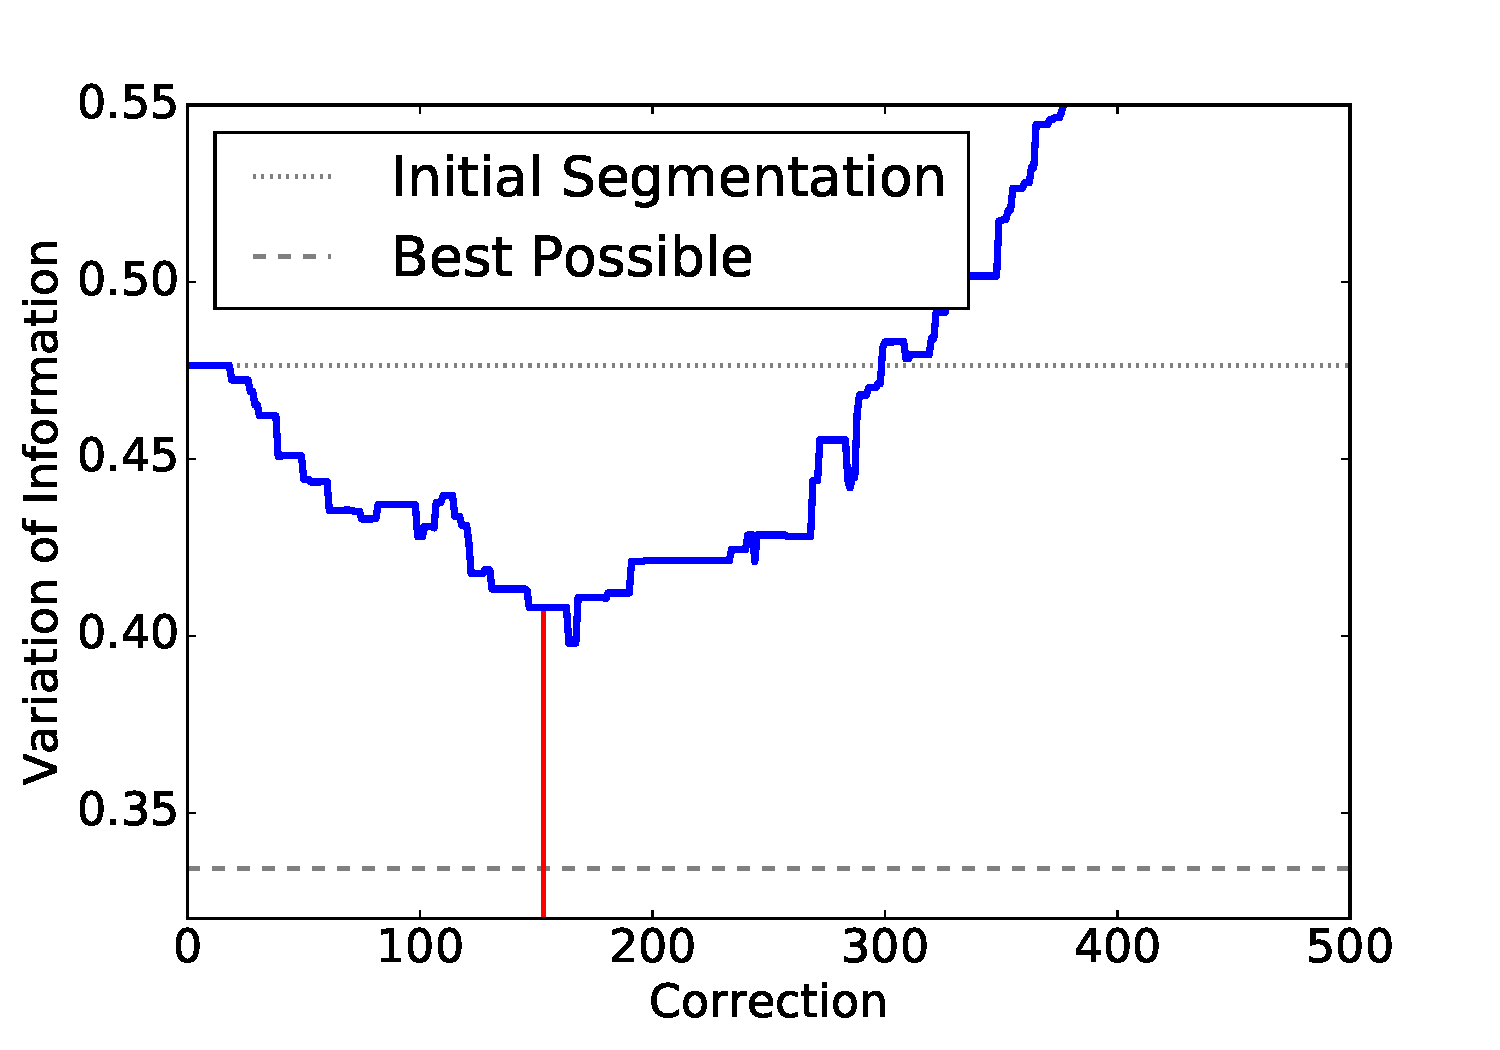
\includegraphics[width=\textwidth]{gfx/gpauto.pdf}
        \caption{A gull}
        \label{fig:gull}
    \end{subfigure}
    ~ %add desired spacing between images, e. g. ~, \quad, \qquad, \hfill etc. 
      %(or a blank line to force the subfigure onto a new line)

    ~ %add desired spacing between images, e. g. ~, \quad, \qquad, \hfill etc. 
    %(or a blank line to force the subfigure onto a new line)
    \begin{subfigure}[b]{0.49\linewidth}
        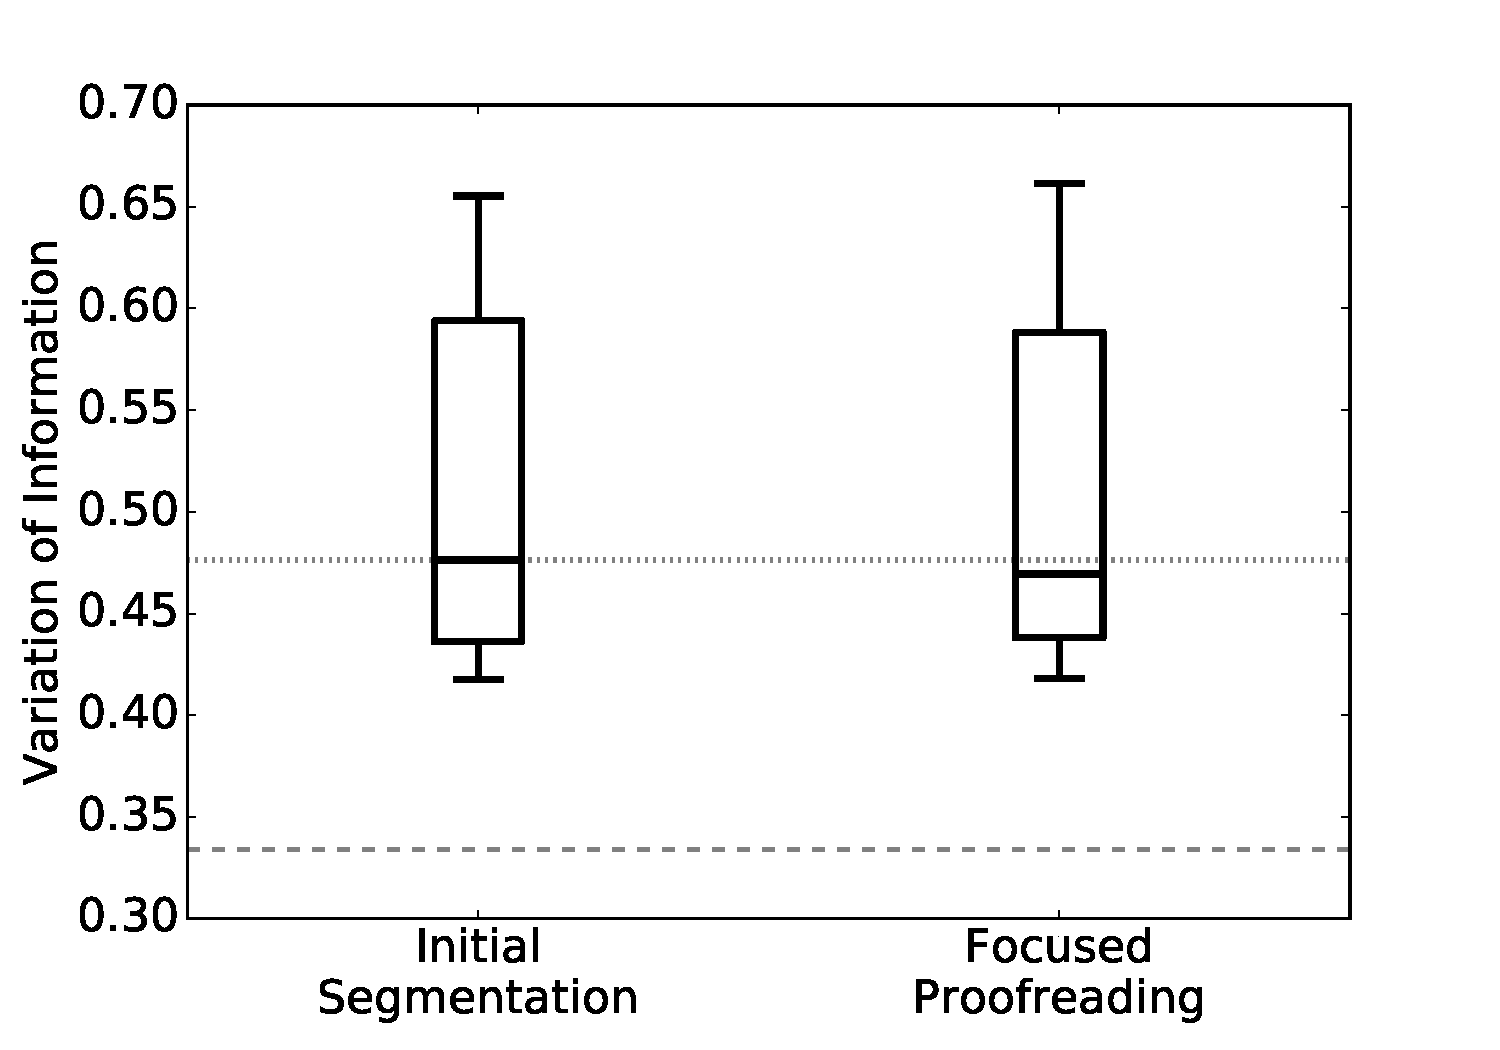
\includegraphics[width=\textwidth]{gfx/fc_fp_ac4.pdf}
        \caption{A mouse}
        \label{fig:mouse}
    \end{subfigure}
    \caption{Pictures of animals}\label{fig:animals}
\end{figure}